%---------------------------PREAMBLE-------------------------------------------- %
\documentclass[9pt]{article}
% \documentclass[9pt]{amsart}
% \documentclass[9pt]{revtex4-2}


%------------------- PACKAGES 

\usepackage{graphicx}
	\graphicspath{ {plots/} }
\usepackage{caption}
\usepackage{epstopdf}
\usepackage{pdfpages}
\usepackage{array}
\usepackage{ulem}
\usepackage{amsfonts}
\usepackage{amssymb}
\usepackage{amsmath}
\usepackage{amsthm}
	\newtheorem{definition}{Definition}[section]
	\newtheorem*{remark}{Remark}
	\newtheorem{theorem}{Theorem}[section]
	\newtheorem{corollary}{Corollary}[theorem]
	\newtheorem{lemma}[theorem]{Lemma}
\usepackage{mathrsfs}
\usepackage{color}
\usepackage{float}
\usepackage{tikz}
\usetikzlibrary{arrows,%
                plotmarks,patterns}
\usepackage{pgfplots}
\pgfplotsset{compat=newest}
\usepgfplotslibrary{fillbetween}

\usepackage{enumerate}
\usepackage{array}
\usepackage{wrapfig}
\usepackage{enumitem}
\usepackage{bm}
\usepackage{booktabs}
\usepackage{siunitx}
\usepackage{authblk}
\usepackage{cancel}
\usepackage{listings}
\usepackage[utf8]{inputenc}

% \usepackage[table]{xcolor}

\usepackage[unicode,psdextra, colorlinks=true, linkcolor=black, citecolor=black, urlcolor=blue, breaklinks]{hyperref}[2012/08/13]


\setlength{\arrayrulewidth}{0.5mm}
% \setlength{\tabcolsep}{10pt}
\renewcommand{\arraystretch}{1.0}


%------------------ USEFULL MACROS ------------------%
%-- MISC
\newcommand{\comment}[1]{}                                % for adding an inline comment
\makeatletter 											  % This entire thing is for redefining *matrix environment in amsmath so that you can specify the line spacing in a matrix by  - \begin{pmatrix}[1.5]
\renewcommand*\env@matrix[1][\arraystretch]{%             
  \edef\arraystretch{#1}%
  \hskip -\arraycolsep
  \let\@ifnextchar\new@ifnextchar
  \array{*\c@MaxMatrixCols c}}
\makeatother

%-- DERIVATIVES
\newcommand{\der}[2]{\frac{\mathrm{d}#1}{\mathrm{d}#2}}          	 % first derivative
\newcommand{\dder}[2]{\frac{\mathrm{d}^{2}#1}{\mathrm{d}#2^{2}}}	 % second derivative
\newcommand{\nder}[3]{\frac{\mathrm{d}^{#3}#1}{\mathrm{d}#2^{#3}}}   % nth derivative
\newcommand{\pder}[2]{\frac{\partial #1}{\partial #2}}               % first partial derivative
\newcommand{\ppder}[2]{\frac{\partial^2 #1}{\partial {#2}^2}}        % second partial derivative
\newcommand{\npder}[3]{\frac{\partial^{#3} #1}{\partial {#2}^{#3}}}  % second partial derivative

%-- SUMMATION
\newcommand{\sumk}[3]{\sum_{#1 = #2}^{#3}}        			% sum over #1 with limits #2 #3
\newcommand{\sumkk}[2]{\sum_{#1, #2} }         	  			% sum over #1 and #2 no limits
\newcommand{\sumkkdom}[3]{\sum_{#1 , #2 \in #3}}   			% sum over #1 and #2 with domain specified

%-- RESEARCH RELATED
\newcommand{\uhat}[1]{\hat{u}_{#1}}      				          % quick fourier mode
\newcommand{\akak}[2]{a_{#1}a_{#2}}      				          % quick convolution amplitudes
\newcommand{\akakak}[3]{\frac{a_{#1}a_{#2}}{a_{#3}}}      	      % quick convolution amplitudes
\newcommand{\triadexpl}[3]{\phi_{#1} + \phi_{#2} - \phi_{#3}}      % quick triad explicitly
\newcommand{\triad}[3]{\varphi_{#1, #2}^{#3}}                     % quick varphi triad
\newcommand{\ii}{\mathrm{i}}      								  % imaginary i
\newcommand{\e}{\mathrm{e}}      								  % e
\newcommand{\Mod}[1]{\ (\mathrm{mod}\ #1)}
\newcommand{\grad}[1]{\nabla{#1}}								% gradient operator
\newcommand{\curl}[1]{\nabla \times {#1}}								% gradient operator
\newcommand{\diverg}[1]{\nabla \cdot {#1}}			% divergence operator
\newcommand{\bfu}{\mathbf{u}}											% vector u in bold font
\newcommand{\omegahat}[1]{\hat{\omega}_{ \mathbf{#1} } }								% gradient operator
\newcommand{\alphakkk}[3]{\alpha_{\bfkn{#1}, \bfkn{#2}}^{\bfkn{#3}}}
\newcommand{\bfx}{\mathbf{x}}								% gradient operator
\newcommand{\bfk}{\mathbf{k}}								% gradient operator
\newcommand{\bfkn}[1]{\mathbf{k}_{#1}}								% gradient operator

%-- COMMENTS / EDITING
\newcommand{\TODO}[1]{\textcolor{red}{TODO: #1}}


%-- CODE SNIPPETS
\newcommand{\code}[1]{\texttt{#1}}





%-------- PAGE STYLE & MARGIN SIZE
% \pagestyle{plain} \setlength{\oddsidemargin}{0.05in}
% \setlength{\evensidemargin}{0.05in} \setlength{\topmargin}{0in}
% \setlength{\footskip}{1.05in} \setlength{\headsep}{0in}
% \setlength{\textwidth}{6.4in} \setlength{\textheight}{8.25in}
\usepackage[a4paper, margin=0.5cm]{geometry}




\title{\textbf{Phase Dynamics - 2D Navier Stokes}}

\author[$1$]{E. M. Carroll}
\author[$1$]{M. D. Bustamante}
\affil[$1$]{Department of Mathematics and Statistics, University College Dublin, Dublin, Ireland} 





\begin{document}


\maketitle	


\section{Enstorphy Flux}

The flux of enstrophy in/out of $\mathcal{C}_{\theta}$ is defined as

\begin{align}
\Pi_{\mathcal{C}_{\theta}} &= 2 \pi^2 \sum_{\substack{\bfkn{3} \in \mathcal{C}_{\theta} \\ \bfkn{1},  \bfkn{2} \in \mathcal{C}_{\theta}^{'} \\ \bfkn{1} + \bfkn{2} = \bfkn{3}}} \left(k_{1 x} k_{2 y}-k_{2 x} k_{1 y}\right)\left(\frac{1}{\left|\mathbf{k}_{1}\right|^{2}}-\frac{1}{\left|\mathbf{k}_{2}\right|^{2}}\right) a_{\mathbf{k}_{1}} a_{\mathbf{k}_{2}} a_{\mathbf{k}_{3}} \cos \left(\varphi_{\mathbf{k}_{1} \mathbf{k}_{2}}^{\mathbf{k}_{3}}\right) \\
&\qquad - 2 \pi^2 \sum_{\substack{\bfkn{1}, \bfkn{2} \in \mathcal{C}_{\theta} \\ \bfkn{3} \in \mathcal{C}_{\theta}^{'} \\ \bfkn{1} + \bfkn{2} = \bfkn{3}}} \left(k_{1 x} k_{2 y}-k_{2 x} k_{1 y}\right)\left(\frac{1}{\left|\mathbf{k}_{1}\right|^{2}}-\frac{1}{\left|\mathbf{k}_{2}\right|^{2}}\right) a_{\mathbf{k}_{1}} a_{\mathbf{k}_{2}} a_{\mathbf{k}_{3}} \cos \left(\varphi_{\mathbf{k}_{1} \mathbf{k}_{2}}^{\mathbf{k}_{3}}\right)
\end{align}

\subsection{Partition of Wavevector Space}

\begin{figure}[H]
 \centering
   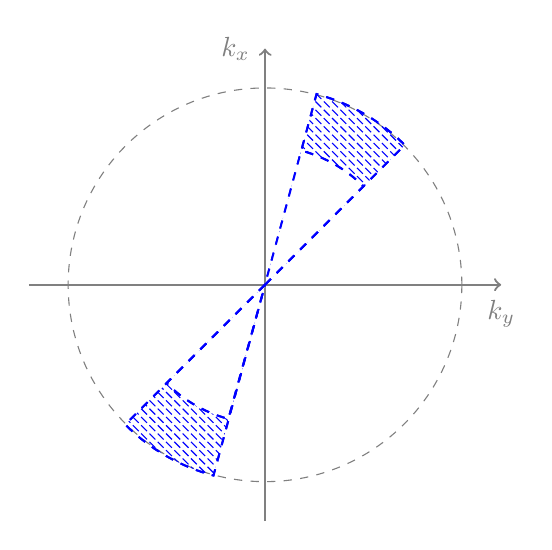
\begin{tikzpicture}
   % Grid
   % \draw [line width=0.5pt, line cap=round, dash pattern=on 0pt off 2\pgflinewidth] (-3,-3) grid (3,3);
    
    Axis
    \draw[thick,->,gray] (-3,0)--(3,0) node[below=1.75pt, fill=white] {$k_y$}; % y axis
    \draw[thick,->,gray] (0,-3)--(0,3) node[left=1.75pt, fill=white] {$k_x$}; % x axis
    
    % Outer Cirlce
    \draw[gray,dashed=onthick] (0,0) circle (2.5cm);

    % -k3 Sector
    \draw[line width=0.25mm,blue,dashed=on 2pt off 3pt, pattern=north west lines, pattern color=blue] (0, 0) -- (-1.775,-1.775) arc[start angle=45 + 180, delta angle=30, radius=2.5cm] -- (0, 0);
    \draw[line width=0.25mm,blue,dashed=on 2pt off 3pt, fill=white] (0, 0) -- (-1.25,-1.25) arc  [start angle=45 + 180, delta angle=30, radius=1.75] -- (0, 0) ;
     \draw[line width=0.25mm,blue,dashed=on 2pt off 3pt] (0, 0) -- (-1.775,-1.775) arc[start angle=45 + 180, delta angle=30, radius=2.5cm] -- (0, 0);
    \draw[line width=0.25mm,blue,dashed=on 2pt off 3pt] (0, 0) -- (-1.25,-1.25) arc  [start angle=45 + 180, delta angle=30, radius=1.75] -- (0, 0) ;
  
    % k3 Sector
    \draw[line width=0.25mm,blue,dashed=on 2pt off 3pt, pattern=north west lines, pattern color=blue] (0,0) -- (1.775,1.775) arc[start angle=45, delta angle=30, radius=2.5cm] -- (0,0);
    \draw[line width=0.25mm,blue,dashed=on 2pt off 3pt, fill=white] (0, 0) -- (1.25,1.25) arc  [start angle=45, delta angle=30, x radius=1.75cm, y radius =1.75cm] ;
    \draw[line width=0.25mm,blue,dashed=on 2pt off 3pt] (0,0) -- (1.775,1.775) arc[start angle=45, delta angle=30, radius=2.5cm] -- (0,0);
    \draw[line width=0.25mm,blue,dashed=on 2pt off 3pt] (0, 0) -- (1.25,1.25) arc  [start angle=45, delta angle=30, x radius=1.75cm, y radius =1.75cm] ;


   \end{tikzpicture}
\end{figure}


Let $\alpha_{\bfkn{1}, \bfkn{2}}^{\bfkn{3}} = \left(k_{1 x} k_{2 y}-k_{2 x} k_{1 y}\right)\left(\frac{1}{\left|\mathbf{k}_{1}\right|^{2}}-\frac{1}{\left|\mathbf{k}_{2}\right|^{2}}\right) a_{\mathbf{k}_{1}} a_{\mathbf{k}_{2}} a_{\mathbf{k}_{3}}$, then we define the following enstrophy flux collective phase for $\mathcal{C}_\theta$

\begin{align}
R_{\mathcal{C}_\theta}\e^{\ii\Phi_{\mathcal{C}_{\theta}}} &= \sum_{\substack{\bfkn{3} \in \mathcal{C}_{\theta} \\ \bfkn{1},  \bfkn{2} \in \mathcal{C}_{\theta}^{'} \\ \bfkn{1} + \bfkn{2} = \bfkn{3}}} \alphakkk{{1}}{2}{3}\e^{\ii \triad{\bfkn{1}}{\bfkn{2}}{\bfkn{3}}} + \sum_{\substack{\bfkn{1}, \bfkn{2} \in \mathcal{C}_{\theta} \\ \bfkn{3} \in \mathcal{C}_{\theta}^{'} \\ \bfkn{1} + \bfkn{2} = \bfkn{3}}} \alphakkk{{1}}{2}{3}\e^{\ii \triad{\bfkn{1}}{\bfkn{2}}{\bfkn{3}}} 
\label{eq:kuramoto_order_param}
\end{align}
where we restrict the summation in the wavevectors to be the right half plane i.e., $k_y > 0$, therefore we only consider the flux into/out of $\mathcal{C}_{\theta}^{+}$. Furthermore the set $\mathcal{C}_{\theta}^{'} \equiv {\mathcal{C}_{\theta}^{+}}^{'}$ can be written as

\begin{align}
	{\mathcal{C}_{\theta}^{+}}^{'} = \bigcup_{\tilde{\theta} \neq \theta} \mathcal{C}_{\tilde{\theta}} \bigcup \mathcal{C}_{\theta}^{L}
\end{align}
where $\mathcal{C}_{\theta}^{L}$ is the lower part of the sector $S_{\theta}$.

Therefore the first term in (\ref{eq:kuramoto_order_param}) becomes

\begin{align}
	\sum_{\substack{\bfkn{3} \in \mathcal{C}_{\theta} \\ \bfkn{1},  \bfkn{2} \in \mathcal{C}_{\theta}^{'} \\ \bfkn{1} + \bfkn{2} = \bfkn{3}}} \alphakkk{{1}}{2}{3}\e^{\ii \triad{\bfkn{1}}{\bfkn{2}}{\bfkn{3}}} &= \sum_{\substack{\bfkn{3} \in \mathcal{C}_{\theta}^{+} \\ \bfkn{1},  \bfkn{2} \in \bigcup_{\tilde{\theta} \neq \theta} \mathcal{C}_{\tilde{\theta}} \bigcup \mathcal{C}_{\theta}^{L} \\ \bfkn{1} + \bfkn{2} = \bfkn{3}}} \alphakkk{{1}}{2}{3}\e^{\ii \triad{\bfkn{1}}{\bfkn{2}}{\bfkn{3}}} \notag \\
	&= \sum_{\tilde{\theta} \neq \theta} \sum_{\substack{\bfkn{3} \in \mathcal{C}_{\theta}^{+} \\ \bfkn{1} \in \mathcal{C}_{\tilde{\theta}} \\ \bfkn{2} \notin \mathcal{C}_{\theta}^{+} \\ \bfkn{1} + \bfkn{2} = \bfkn{3}}} \alphakkk{{1}}{2}{3}\e^{\ii \triad{\bfkn{1}}{\bfkn{2}}{\bfkn{3}}} + \sum_{\substack{\bfkn{3} \in \mathcal{C}_{\theta}^{+} \\ \bfkn{1} \in \mathcal{C}_{\theta}^{L} \\ \bfkn{2} \notin \mathcal{C}_{\theta}^{+} \\ \bfkn{1} + \bfkn{2} = \bfkn{3}}} \alphakkk{{1}}{2}{3}\e^{\ii \triad{\bfkn{1}}{\bfkn{2}}{\bfkn{3}}}
\end{align}

and the second term in (\ref{eq:kuramoto_order_param}) becomes

\begin{align}
	\sum_{\substack{\bfkn{1}, \bfkn{2} \in \mathcal{C}_{\theta} \\ \bfkn{3} \in \mathcal{C}_{\theta}^{'} \\ \bfkn{1} + \bfkn{2} = \bfkn{3}}} \alphakkk{{1}}{2}{3}\e^{\ii \triad{\bfkn{1}}{\bfkn{2}}{\bfkn{3}}} &= \sum_{\substack{\bfkn{1}, \bfkn{2} \in \mathcal{C}_{\theta}^{+} \\ \bfkn{3} \in \bigcup_{\tilde{\theta} \neq \theta} \mathcal{C}_{\tilde{\theta}} \bigcup \mathcal{C}_{\theta}^{L} \\ \bfkn{1} + \bfkn{2} = \bfkn{3}}} \alphakkk{{1}}{2}{3}\e^{\ii \triad{\bfkn{1}}{\bfkn{2}}{\bfkn{3}}} \notag \\
	&= \sum_{\tilde{\theta} \neq \theta} \sum_{\substack{\bfkn{1}, \bfkn{2} \in \mathcal{C}_{\theta}^{+} \\ \bfkn{3} \in \mathcal{C}_{\tilde{\theta}} \\ \bfkn{1} + \bfkn{2} = \bfkn{3}}} \alphakkk{{1}}{2}{3}\e^{\ii \triad{\bfkn{1}}{\bfkn{2}}{\bfkn{3}}} + \sum_{\substack{\bfkn{1}, \bfkn{2} \in \mathcal{C}_{\theta}^{+} \\ \bfkn{3} \in \mathcal{C}_{\theta}^{L} \\ \bfkn{1} + \bfkn{2} = \bfkn{3}}} \alphakkk{{1}}{2}{3}\e^{\ii \triad{\bfkn{1}}{\bfkn{2}}{\bfkn{3}}}
\end{align}

Therefore to obtian the flux into/out of $\mathcal{C}_{\theta}^{+}$ we have

\begin{align}
	\Pi_{\mathcal{C}_{\theta}^{+}} = \sum_{\tilde{\theta} \neq \theta} \left( \sum_{\substack{\bfkn{3} \in \mathcal{C}_{\theta}^{+} \\ \bfkn{1} \in \mathcal{C}_{\tilde{\theta}} \\ \bfkn{2} \notin \mathcal{C}_{\theta}^{+} \\ \bfkn{1} + \bfkn{2} = \bfkn{3}}} \alphakkk{{1}}{2}{3}\e^{\ii \triad{\bfkn{1}}{\bfkn{2}}{\bfkn{3}}} + \sum_{\substack{\bfkn{1}, \bfkn{2} \in \mathcal{C}_{\theta}^{+} \\ \bfkn{3} \in \mathcal{\tilde{\theta}} \\ \bfkn{1} + \bfkn{2} = \bfkn{3}}} \alphakkk{{1}}{2}{3}\e^{\ii \triad{\bfkn{1}}{\bfkn{2}}{\bfkn{3}}} \right) +  \sum_{\substack{\bfkn{3} \in \mathcal{C}_{\theta}^{+} \\ \bfkn{1} \in \mathcal{C}_{\theta}^{L} \\ \bfkn{2} \notin \mathcal{C}_{\theta}^{+} \\ \bfkn{1} + \bfkn{2} = \bfkn{3}}} \alphakkk{{1}}{2}{3}\e^{\ii \triad{\bfkn{1}}{\bfkn{2}}{\bfkn{3}}} + \sum_{\substack{\bfkn{1}, \bfkn{2} \in \mathcal{C}_{\theta}^{+} \\ \bfkn{3} \in \mathcal{C}_{\theta}^{L} \\ \bfkn{1} + \bfkn{2} = \bfkn{3}}} \alphakkk{{1}}{2}{3}\e^{\ii \triad{\bfkn{1}}{\bfkn{2}}{\bfkn{3}}}
\end{align}


which can be loosely interpretted as sum of the contributions to the flux in 1D (along the sector $S_\theta$) and contributions to the flux in 2D which is a function of the angles $\theta$ (denoting the sector that $\bfkn{3}$ lies in) and $\tilde{\theta}$ (the sector that $\bfkn{1}$ lies in)
	
\begin{align}
	\Pi_{\mathcal{C}_{\theta}^{+}} = \sum_{\tilde{\theta} \neq \theta} \Pi_{\text{2D}}(\theta, \tilde{\theta}) + \Pi_{\text{1D}}
\end{align}
and this term can be validated against the flux computed using the nonlinear term of the equations of motion where you consider only the flux contained in the modes in $\mathcal{C}_{\theta}^{+}$

\begin{align}
	\Pi_{\mathcal{C}_{\theta}^{+}} \simeq \der{}{t} \sum_{\bfk \in \mathcal{C}_{\theta}^{+}} |\omega_{\bfk}|^2
\end{align}


\end{document}